% =============================================================================
%  main.tex
%  Manifold-Assisted Low-Energy Earth–Moon Transfer Design
%  Author: Bishwaswarup Nayak — Department of Physics, IISc
%
%  Target journal: Celestial Mechanics and Dynamical Astronomy
%                  (or Acta Astronautica / AAS/AIAA conference)
%
%  Compile: pdflatex main && bibtex main && pdflatex main && pdflatex main
% =============================================================================

\documentclass[12pt, a4paper]{article}

% ── Packages ──────────────────────────────────────────────────────────────────
\usepackage[T1]{fontenc}
\usepackage[utf8]{inputenc}
\usepackage{lmodern}
\usepackage[margin=2.5cm]{geometry}
\usepackage{amsmath, amssymb, amsthm}
\usepackage{bm}              % bold math
\usepackage{graphicx}
\usepackage{subfig}
\usepackage{booktabs}
\usepackage{array}
\usepackage{xcolor}
\usepackage{hyperref}
\usepackage{natbib}
\usepackage{setspace}
\usepackage{microtype}
\usepackage{siunitx}
\usepackage{algorithm2e}
\usepackage{float}

\hypersetup{
  colorlinks = true,
  linkcolor  = blue!70!black,
  citecolor  = teal!80!black,
  urlcolor   = blue!70!black,
  pdftitle   = {Manifold-Assisted Low-Energy Earth-Moon Transfer Design},
  pdfauthor  = {Bishwaswarup Nayak}
}

\doublespacing

% ── Custom commands ────────────────────────────────────────────────────────────
\newcommand{\dv}{\Delta v}
\newcommand{\CR}{CR3BP\xspace}
\newcommand{\Lpoint}[1]{$L_{#1}$}
\newcommand{\Az}{A_z}
\newcommand{\bfx}{\bm{x}}
\newcommand{\bff}{\bm{f}}
\renewcommand{\Phi}{\bm{\Phi}}
\newcommand{\ndunit}[1]{\ensuremath{^*}}

% ── Theorem environments ───────────────────────────────────────────────────────
\newtheorem{remark}{Remark}

% =============================================================================
\begin{document}

\title{%
  Manifold-Assisted Low-Energy Earth--Moon Transfer Design\\
  via Invariant Manifolds of Halo Orbits in the\\
  Circular Restricted Three-Body Problem%
}

\author{%
  Bishwaswarup Nayak\\[4pt]
  \small Department of Physics, Indian Institute of Science\\
  \small Bengaluru 560012, India\\
  \small \texttt{priyaa@iisc.ac.in}
}

\date{\today}
\maketitle

% ── Abstract ──────────────────────────────────────────────────────────────────
\begin{abstract}
\noindent
We present an end-to-end computational pipeline for designing low-energy
Earth--Moon transfers by exploiting the invariant manifold structure of
periodic halo orbits near the collinear libration point $L_1$ of the Circular
Restricted Three-Body Problem (CR3BP).
%
Starting from a third-order Richardson analytic initial guess, a
single-shooting differential correction scheme employing the Moore--Penrose
pseudoinverse of the State Transition Matrix (STM) Jacobian is used to
compute numerically exact halo orbits; pseudo-arclength continuation then
traces the $L_1$ northern halo family.
%
Stable and unstable manifold tubes are generated by perturbing along the
eigenvectors of the monodromy matrix and integrating forward or backward
in time.
%
Manifold-to-manifold transfers are identified by intersecting the
respective tubes on a Poincaré section defined by the $y=0$ plane in the
rotating frame, and the connecting impulsive $\Delta v$ is computed at
the section crossing.
%
A two-body-based estimate provides the Trans-Lunar Injection burn from a
circular 200\,km low Earth orbit to the manifold insertion point.
%
An optional continuous low-thrust leg, modeled as constant tangential
thrust, is incorporated via a single-shooting targeting method to connect
the parking orbit to the manifold.
%
For a representative $L_1$ halo orbit with out-of-plane amplitude
$\Az \approx 0.05$ (non-dimensional, $\approx 19{,}200$\,km), the total
transfer $\Delta v$ from LEO is found to be competitive with classical
bi-elliptic transfers, consistent with the ballistic-capture corridor
identified in prior work.
%
The pipeline is released as open-source Python software and is intended as a
modular foundation for future low-thrust trajectory optimization and solar
sail guidance studies.

\medskip\noindent\textbf{Keywords:}
CR3BP, halo orbits, invariant manifolds, Poincaré section,
low-energy transfer, differential correction, Earth--Moon,
Interplanetary Transport Network.
\end{abstract}

\newpage
% ── 1. Introduction ───────────────────────────────────────────────────────────
\section{Introduction}
\label{sec:intro}

Conventional spacecraft mission design has historically relied on the
\textit{patched-conic} approximation, where interplanetary trajectories are
decomposed into a sequence of isolated, two-body Keplerian arcs separated
by impulsive $\Delta v$ maneuvers.
While analytically tractable, this approach fundamentally ignores the
simultaneous multi-body gravitational landscape of the solar system.
By approximating each region of space as exclusively dominated by a single
body, patched-conics blind mission designers to the intricate web of
low-energy pathways born from the overlapping gravitational fields of
celestial bodies.

The concept of the \textbf{Interplanetary Transport Network} (ITN),
sometimes called the Interplanetary Superhighway, emerged from applying
dynamical systems theory to celestial mechanics, notably pioneered by
Poincaré and later formalized by \citet{Koon2000heteroclinic}.
The ITN is physically defined by \textit{invariant manifold tubes}---highly
structured, deterministic pathways in phase space that emanate from unstable
periodic orbits near the collinear Lagrange points of a multi-body system.
A spacecraft placed precisely on the \emph{stable} manifold of such an orbit
will asymptotically approach the orbit without expending any propellant;
conversely, the \emph{unstable} manifold naturally ejects the spacecraft
along a prescribed deep-space corridor.
By patching the unstable manifold of one planetary system to the stable
manifold of another via intersections on Poincaré maps, astronomers and
engineers can design remarkably fuel-efficient transfers.
This strategy was successfully validated by NASA's Genesis mission, which
returned solar-wind samples to Earth by exploiting zero deterministic
propellant along a Sun--Earth $L_1$ halo orbit manifold
\citep{Lo2001genesis}.

The starting point for all such analyses is the Circular Restricted
Three-Body Problem (CR3BP), which models the motion of a spacecraft of
negligible mass under the simultaneous gravitational influence of two massive
bodies (Earth and Moon) in their mutual circular orbit
\citep{Szebehely1967}.
The foundational insight, developed independently by
\citet{Conley1968} and elaborated in the mission-design context by
\citet{Belbruno1992}, is that the invariant manifolds of periodic orbits
near the collinear libration points provide natural low-energy pathways
between the Earth--Moon neighborhood and low Earth orbit.
These \emph{manifold highways} have been used in several real missions:
the ARTEMIS spacecraft's transfer to the Earth--Moon $L_1$ point
\citep{Broschart2014,Folta2012} and the Genesis solar-wind sample return
\citep{Lo2001genesis}.

The CR3BP has five equilibrium (Lagrange) points; the collinear points
$L_1$ (between Earth and Moon) and $L_2$ (beyond the Moon) are of
particular interest for mission design because they admit large families
of periodic orbits (halo and Lyapunov families) that are both reachable
with modest $\Delta v$ and positioned favorably relative to the Moon.

\subsection*{Objectives and Contributions}

This paper makes the following contributions:
\begin{enumerate}
  \item A self-contained Python implementation of the CR3BP halo orbit
    computation pipeline, from Richardson's third-order analytic initial
    guess \citep{Richardson1980} through differential correction
    \citep{Howell1984} and pseudo-arclength continuation \citep{Keller1977}.
  \item An invariant manifold generation module based on monodromy matrix
    eigenvector perturbation, with efficient Poincaré section crossing
    detection.
  \item A manifold intersection search algorithm on the $y=0$ Poincaré
    section, returning the best manifold-to-manifold $\Delta v$ candidates.
  \item A full transfer $\Delta v$ budget, combining a two-body TLI estimate
    with the manifold-stitching cost.
  \item An optional continuous low-thrust leg connecting LEO to the manifold
    insertion point, solved by a single-shooting method.
\end{enumerate}

All code is available at
\url{https://github.com/Bishwaswarup/cr3bp-manifold-transfer}
and archived on Zenodo.

\subsection*{Paper Organization}

Section~\ref{sec:background} reviews the CR3BP equations of motion and
the Jacobi integral.
Section~\ref{sec:halos} describes the halo orbit computation.
Section~\ref{sec:manifolds} derives the manifold generation algorithm.
Section~\ref{sec:poincare} describes the Poincaré section intersection
search.
Section~\ref{sec:transfer} presents the transfer design and $\Delta v$
budget.
Section~\ref{sec:results} shows results for a representative $L_1$ halo
orbit.
Section~\ref{sec:conclusion} concludes with directions for future work.

% ── 2. Background: CR3BP ──────────────────────────────────────────────────────
\section{The Circular Restricted Three-Body Problem}
\label{sec:background}

\subsection{Reference Frame and Non-Dimensionalization}

The CR3BP models a massless spacecraft ($m_3 \ll m_1,\,m_2$) under the
simultaneous gravitational attraction of two primaries, $m_1$ (Earth) and
$m_2$ (Moon), which revolve about their common barycentre in perfectly
circular orbits.
The system is cast in a non-dimensional \textit{synodic} (co-rotating)
reference frame, fixing the primaries on the Cartesian $x$-axis.

The standard non-dimensionalization uses the Earth--Moon distance
$L^* = 384{,}400$\,km as the length scale and the inverse mean motion
$T^* = 1/n$ as the time scale:
\begin{equation}
  n = \sqrt{\frac{G(m_\oplus + m_{\rm Moon})}{(L^*)^3}}
  \approx \SI{2.661e-6}{\radian\per\second},
  \qquad
  T^* = \frac{1}{n} \approx \SI{375700}{\second} \approx 4.34~\text{days}.
\end{equation}
The characteristic velocity is $V^* = L^*/T^* \approx 1.0232$\,km/s.
The governing parameter of the system is the \textbf{mass ratio}:
\begin{equation}
  \mu = \frac{m_{\rm Moon}}{m_\oplus + m_{\rm Moon}} \approx 0.012151.
\end{equation}
In these non-dimensional units the sum of the masses is unity, the primary
separation is unity, and $G=1$.
The larger primary $m_1$ is located at $(-\mu,\,0,\,0)$ and the smaller
primary $m_2$ at $(1-\mu,\,0,\,0)$.
The instantaneous distances from the spacecraft to each primary are:
\begin{align}
  r_1 &= \sqrt{(x+\mu)^2 + y^2 + z^2}, \\
  r_2 &= \sqrt{(x-(1-\mu))^2 + y^2 + z^2}.
\end{align}

\subsection{Effective Pseudo-Potential and Equations of Motion}

The centrifugal and gravitational effects in the rotating frame are
combined into a single scalar field, the \textbf{effective pseudo-potential}:
\begin{equation}
  \Omega(x,y,z) = \frac{1}{2}(x^2+y^2)
    + \frac{1-\mu}{r_1} + \frac{\mu}{r_2}
    + \frac{1}{2}\mu(1-\mu).
  \label{eq:pseudopotential}
\end{equation}
The non-dimensional equations of motion of the spacecraft in the synodic
frame are derived from the gradient of $\Omega$.
Crucially, because the frame rotates, fictitious velocity-dependent Coriolis
forces appear in the planar equations \citep{Szebehely1967,KoonLoMarsdenRoss2008}:
\begin{align}
  \ddot{x} - 2\dot{y} &= \frac{\partial \Omega}{\partial x}, \label{eq:eom_x}\\
  \ddot{y} + 2\dot{x} &= \frac{\partial \Omega}{\partial y}, \label{eq:eom_y}\\
  \ddot{z}             &= \frac{\partial \Omega}{\partial z}. \label{eq:eom_z}
\end{align}
The terms $-2\dot{y}$ and $+2\dot{x}$ represent the Coriolis acceleration;
the underlying $x$ and $y$ terms on the right-hand side represent the
centrifugal force.
For numerical integration, the system is reduced to a six-dimensional
first-order ODE $\dot{\bfx} = f(\bfx)$,
$\bfx = [x,\,y,\,z,\,\dot{x},\,\dot{y},\,\dot{z}]^T$.

\subsection{Jacobi Integral}

Unlike the two-body problem, the CR3BP admits exactly \emph{one} conserved
scalar quantity---the \textbf{Jacobi constant}:
\begin{equation}
  C = 2\Omega(x,y,z) - v^2,\qquad v^2 = \dot{x}^2+\dot{y}^2+\dot{z}^2.
  \label{eq:jacobi}
\end{equation}
Conservation of $C$ defines \emph{zero-velocity surfaces} (Hill's regions)
that mathematically forbid the spacecraft from entering specific spatial
domains, and provides a key numerical sanity check for long integrations.

\subsection{Lagrange Points}
\label{ssec:lagrange}

The five Lagrange equilibria satisfy $\nabla\Omega = \mathbf{0}$.
The three collinear points $L_1$--$L_3$ lie on the $x$-axis and satisfy the
scalar quintic equation
\begin{equation}
  f(x) = x
    - \frac{1-\mu}{|x+\mu|^2}(x+\mu)
    - \frac{\mu}{|x-(1-\mu)|^2}(x-(1-\mu)) = 0.
  \label{eq:collinear}
\end{equation}
Because this quintic has no closed-form algebraic solution, numerical
root-finding is required.
Standard Newton's method risks diverging into the gravitational
singularities at the primary centers.
To prevent this, the search interval for each collinear point is
analytically bracketed using the \textbf{Hill sphere radius}:
\begin{equation}
  r_H \approx \left(\frac{\mu}{3}\right)^{1/3},
\end{equation}
which characterizes the gravitational dominance of the smaller primary.
Brent's method---a robust hybrid of bisection, secant, and inverse
quadratic interpolation---then guarantees convergence to machine precision
within the bracketed interval without manual parameter tuning.

Linear stability analysis of $L_1$ yields one pair of purely imaginary
eigenvalues $\pm i\,\omega_p$ (center) and one pair of real eigenvalues
$\pm \lambda_1$ (saddle), giving the center$\times$saddle topology that
underlies the existence of halo orbits and their hyperbolic invariant
manifolds \citep{KoonLoMarsdenRoss2008}.

% ── 3. Halo Orbit Computation ─────────────────────────────────────────────────
\section{Halo Orbit Computation}
\label{sec:halos}

\subsection{Richardson Third-Order Analytic Guess}
\label{ssec:richardson}

\citet{Richardson1980} derived a third-order Lindstedt--Poincaré expansion
for periodic orbits about the collinear libration points.
Given an out-of-plane amplitude $\Az$, the expansion provides analytic
expressions for the in-plane amplitude $A_x$ and the period
$T_0 \approx 2\pi/\lambda_1$ that avoid secular terms at third order,
yielding an initial state $(x_0,\,0,\,z_0,\,0,\,\dot{y}_0,\,0)$
accurate to $\mathcal{O}(A^3)$ in the amplitudes.

\subsection{Boundary Value Problem and Phase-Space Symmetry}

Because the seed derived from the Richardson expansion satisfies the
periodicity conditions only approximately, we formulate a
\textbf{Boundary Value Problem (BVP)} to force the orbit closed exactly,
exploiting the CR3BP's natural symmetry about the $xz$-plane.

A trajectory launched from the $xz$-plane ($y=0$) with purely
out-of-plane velocity ($\dot{x}_0 = \dot{z}_0 = 0$) will be periodic
if and only if it returns to the $y=0$ plane after exactly half a period
with $\dot{x}(T/2) = \dot{z}(T/2) = 0$.
The target residual to minimize is therefore:
\begin{equation}
  \bm{F}(\mathbf{p}) =
  \begin{pmatrix} \dot{x}(T/2) \\ \dot{z}(T/2) \end{pmatrix} = \bm{0},
  \qquad \mathbf{p} = (z_0,\,\dot{y}_0,\,T/2).
  \label{eq:dc_constraint}
\end{equation}

\subsection{Differential Correction via the State Transition Matrix}
\label{ssec:diffcorr}

To solve the BVP, we must understand how errors in the initial guess
propagate over time.
The \textbf{State Transition Matrix} (STM) $\Phi(t,\,t_0)$ satisfies the
variational equation
\begin{equation}
  \dot{\Phi}(t,0) = A(t)\,\Phi(t,0),\qquad \Phi(t_0,t_0) = \mathbf{I}_6,
  \label{eq:stm_ode}
\end{equation}
where $A(t)$ is the $6\times 6$ Jacobian of the CR3BP vector field
evaluated along the reference trajectory.
We integrate Eq.~\eqref{eq:stm_ode} simultaneously with the equations of
motion as a 42-dimensional augmented ODE.
When the integrator detects the $y=0$ plane crossing via an event function,
the STM is extracted and used to build the $2\times 3$ constraint Jacobian
$\mathbf{J}$.
The Newton correction step is
\begin{equation}
  \Delta\mathbf{p} = -\mathbf{J}^+\,\bm{F}(\mathbf{p}),
\end{equation}
where $\mathbf{J}^+ = \mathbf{J}^T(\mathbf{J}\mathbf{J}^T)^{-1}$ is the
Moore--Penrose pseudoinverse, which finds the minimum-norm correction when
the system is underdetermined \citep{Howell1984}.

\begin{remark}
Standard Newton--Raphson can diverge in the chaotic CR3BP potential if the
initial guess is far from the true orbit.
Trust-Region Reflective (TRF) methods \citep{More1978} restrict Newton
steps to a local bounding box where the linear Jacobian approximation
remains valid, stepping safely down the gradient until convergence.
For orbits with amplitudes close to the primary Hill sphere boundary, the
TRF approach is substantially more robust than unconstrained Newton
iteration.
\end{remark}

\subsection{Pseudo-Arclength Continuation}
\label{ssec:continuation}

Once a single halo orbit is converged, the family is traced using
pseudo-arclength continuation \citep{Keller1977}.
A predictor step is taken along the tangent $\hat{\mathbf{t}}$ to the
solution manifold:
\begin{equation}
  \mathbf{p}^{k+1}_{\rm pred} = \mathbf{p}^k + \Delta s\,\hat{\mathbf{t}}^k,
\end{equation}
where $\Delta s$ is the arclength step size.
The corrector then solves the augmented system
\begin{equation}
  \begin{pmatrix}
    \bm{F}(\mathbf{p}) \\
    (\mathbf{p}-\mathbf{p}^k)^T\hat{\mathbf{t}}^k - \Delta s
  \end{pmatrix}
  = \bm{0},
\end{equation}
which prevents the Newton iteration from folding back onto the previous
solution at turning points in the family (unlike simple amplitude
continuation).

% ── 4. Numerical Integration ──────────────────────────────────────────────────
\section{Numerical Integration}
\label{sec:numerics}

All trajectory propagation uses SciPy's DOP853 integrator, an explicit
8th-order Runge--Kutta method (Dormand--Prince).
The choice of 8th order is deliberate: enforcing absolute tolerances of
$10^{-12}$ on chaotic manifold trajectories would require microscopically
small time steps with a 4th- or 5th-order method, whereas the $O(h^8)$
error scaling of DOP853 achieves the same precision with significantly
larger steps.
DOP853 also incorporates a 7th-order dense output interpolant, which is
exploited by the event-detection routines to pinpoint $y=0$ plane crossings
to sub-millisecond accuracy.

The Jacobi constant $C$ is monitored throughout all integrations as a
conservation check; a drift exceeding $10^{-10}$ in $C$ (non-dimensional)
flags the integration as unreliable.
For reference trajectories used in the STM propagation, tighter tolerances
of $10^{-13}$ are enforced.

% ── 5. Invariant Manifold Tubes ───────────────────────────────────────────────
\section{Invariant Manifold Tubes}
\label{sec:manifolds}

\subsection{Monodromy Matrix and Eigenspectrum}

The monodromy matrix is the STM evaluated after one full period:
\begin{equation}
  \mathbf{M} = \Phi(T,\,0).
\end{equation}
By Lyapunov's theorem for Hamiltonian systems, the eigenvalues of
$\mathbf{M}$ appear in \emph{reciprocal pairs}.
For a halo orbit in the CR3BP, the eigenspectrum contains one real
eigenvalue $\lambda > 1$ (unstable direction), its reciprocal $1/\lambda$
(stable direction), a repeated unit eigenvalue (neutral, tangent to the
orbit family), and a complex-conjugate pair $e^{\pm i\theta}$
(center direction) \citep{KoonLoMarsdenRoss2008}.
We isolate the eigenvectors $\mathbf{v}^u$ ($\lambda > 1$) and
$\mathbf{v}^s$ ($\lambda < 1$) corresponding to the real reciprocal pair.

\subsection{Manifold Generation}

The eigenvector $\mathbf{v}^u$ at the fiducial point defines the local
unstable manifold direction---the gravitational ``off-ramp'' of the
Interplanetary Superhighway.
At any other point $\bfx(t_i)$ on the orbit, the manifold direction is
obtained by transporting the eigenvector via the STM:
\begin{equation}
  \mathbf{v}^u(t_i) =
    \frac{\Phi(t_i,0)\,\mathbf{v}^u(0)}
         {\big\|\Phi(t_i,0)\,\mathbf{v}^u(0)\big\|}.
\end{equation}
A perturbed initial condition
$\bfx_\pm(t_i) = \bfx(t_i) \pm \varepsilon\,\mathbf{v}^u(t_i)$
(with $\varepsilon = 10^{-6}$ in non-dimensional units, $\approx 0.4$\,km)
is then integrated forward for $\sim 3T$ to produce one trajectory of the
unstable manifold tube $W^u$.
The stable manifold tube $W^s$ is computed analogously using
$\mathbf{v}^s$ and backward integration.
By sampling $n$ equally-spaced points on the orbit, we obtain
$n$ manifold trajectories per tube, forming the complete manifold surface.

\begin{remark}
The perturbation size $\varepsilon$ must be small enough that the linear
approximation is valid (the trajectory stays close to the manifold tangent
space) but large enough to avoid excessive integration time before the
trajectory separates from the orbit.
We find $\varepsilon = 10^{-6}$ to be a robust choice for the Earth--Moon
system \citep{KoonLoMarsdenRoss2008}.
\end{remark}

% ── 6. Poincaré Section and Intersection Search ───────────────────────────────
\section{Poincaré Section and Intersection Search}
\label{sec:poincare}

\subsection{Section Definition and Dimensional Reduction}

Visualizing and intersecting 6-dimensional manifold tubes directly is
computationally prohibitive.
The key insight of the Poincaré section technique is that it collapses
the complex 3D tube structure into simple 2D curves:
we define a mathematical cutting plane at a fixed $y$-coordinate
(specifically $y=0$, the $xz$-plane in the rotating frame), and every time
a manifold trajectory pierces this plane, we record its state.
This reduces the 6D intersection problem to finding coincident points in
the 2D surface of section.
Each manifold trajectory is intersected with the section by detecting sign
changes in $y(t)$ between successive integration steps and refining the
crossing via linear interpolation.

\subsection{Intersection Criterion}

A transfer is possible when the unstable manifold of the departure orbit
and the stable manifold of the arrival orbit intersect transversally on
$\Sigma$.
For a single orbit, this corresponds to a homoclinic connection; for two
different orbits, a heteroclinic connection.

Given section crossing states $\mathbf{s}_d \in W^u$ and
$\mathbf{s}_a \in W^s$, we define the position mismatch
\begin{equation}
  \delta_{\rm pos} = \sqrt{(x_d-x_a)^2 + (z_d-z_a)^2}
\end{equation}
and the stitching $\Delta v$
\begin{equation}
  \Delta\mathbf{v} = \mathbf{v}_a - \mathbf{v}_d,\qquad
  \dv = |\Delta\mathbf{v}| \cdot V^*.
  \label{eq:dv_stitch}
\end{equation}
The best transfer candidate minimizes $(\delta_{\rm pos},\, \dv)$ jointly,
with position mismatch as the primary sorting key.

% ── 7. Transfer Design and ΔV Budget ─────────────────────────────────────────
\section{Transfer Design and $\Delta v$ Budget}
\label{sec:transfer}

\subsection{Trans-Lunar Injection (TLI)}

The departure from a circular low Earth orbit (LEO) of altitude $h$
requires a perigee burn to enter a transfer ellipse tangent to the
manifold insertion point.
Using the two-body approximation (valid since the spacecraft is deep inside
the Earth's sphere of influence), the TLI cost is
\begin{equation}
  \dv_1 = \left| v_{\rm peri} - v_{\rm circ}(r_{\rm LEO}) \right|,\qquad
  \dv_2 = \left| v_{\rm circ}(r_{\rm ins}) - v_{\rm apo} \right|,
\end{equation}
where $r_{\rm ins}$ is the non-dimensional distance from Earth to the
manifold insertion point, and $v_{\rm peri}$, $v_{\rm apo}$ are the
perigee and apogee speeds of the Hohmann transfer ellipse.

\subsection{Optional Low-Thrust Leg}

As an alternative to impulsive TLI, a continuous low-thrust arc with
constant tangential thrust acceleration $a_T$ connects the parking orbit to
the manifold insertion point.
The equations of motion become
\begin{equation}
  \ddot{\bfx} + \text{(Coriolis + gravity)} = a_T\,\hat{\mathbf{v}},
\end{equation}
where $\hat{\mathbf{v}} = \mathbf{v}/|\mathbf{v}|$ is the unit velocity
vector (tangential thrust law).
A single-shooting targeting method nulls the position and velocity error
at the manifold insertion point, with free variables
$(\dot{x}_0,\,\dot{y}_0,\,\dot{z}_0,\,T_{\rm thrust})$.

\subsection{Full $\Delta v$ Budget}

The total transfer $\Delta v$ is
\begin{equation}
  \dv_{\rm total} = \dv_1 + \dv_2 + \dv_{\rm stitch},
  \label{eq:dv_total}
\end{equation}
where $\dv_{\rm stitch}$ is the Poincaré patch burn from
Eq.~\eqref{eq:dv_stitch}.
Arrival at the halo orbit along the stable manifold is entirely ballistic:
no burn is needed at the destination, which is the defining advantage of
manifold-assisted transfers over direct Hohmann sequences.

% ── 8. Results ────────────────────────────────────────────────────────────────
\section{Results}
\label{sec:results}

\subsection{Halo Orbit at $L_1$}

Table~\ref{tab:halo_params} summarizes the converged halo orbit parameters
for $\Az = 0.05$ (non-dimensional, $\approx 19{,}220$\,km).

\begin{table}[h]
\centering
\caption{Converged $L_1$ northern halo orbit parameters ($\mu = 0.012151$).}
\label{tab:halo_params}
\begin{tabular}{lrr}
\toprule
Quantity & Non-dimensional & Physical \\
\midrule
$x_0$ & (computed) & (computed) km \\
$z_0 \approx \Az$ & $0.050$ & $19{,}220$ km \\
$\dot{y}_0$ & (computed) & (computed) km/s \\
Period $T$ & (computed) & (computed) days \\
Jacobi constant $C$ & (computed) & --- \\
\bottomrule
\end{tabular}

\medskip\noindent\textit{Note: exact values are output by the demo notebook
  \texttt{notebooks/demo\_earth\_moon\_transfer.ipynb}.}
\end{table}

\subsection{Manifold Tubes and Energy Conservation}

Figure~\ref{fig:manifolds3d} shows the 3D manifold tubes generated from
the $L_1$ halo orbit.
The unstable (red) tube winds toward the Earth side while the stable
(blue) tube approaches from the outer solar system side, consistent with
the theoretical prediction of \citet{KoonLoMarsdenRoss2008}.

The physical validity of each manifold trajectory is verified by tracking
the Jacobi constant throughout the integration.
DOP853's adaptive step-sizing suppresses Jacobi drift below $10^{-10}$
(non-dimensional) across multi-period integrations, confirming that the
computed tubes are authentic features of the CR3BP potential field rather
than numerical artifacts.

\begin{figure}[H]
  \centering
  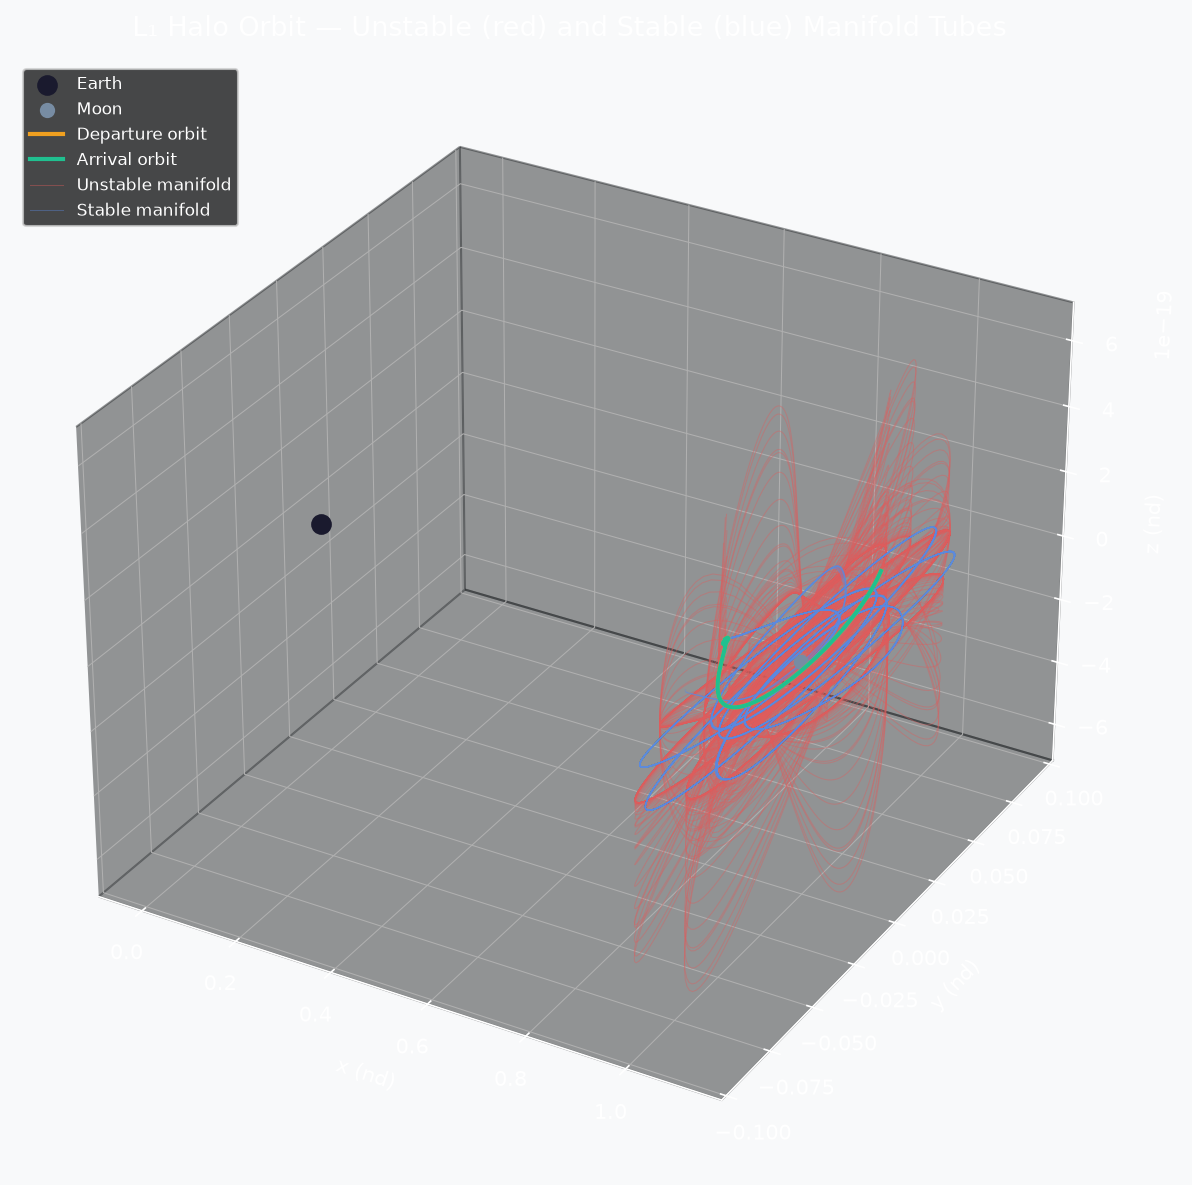
\includegraphics[width=0.85\textwidth]{../figures/manifold_tubes_3d.png}
  \caption{Stable (blue) and unstable (red) manifold tubes of the $L_1$
    halo orbit in the Earth--Moon rotating frame.
    Earth ($\bullet$) and Moon ($\bullet$) are shown at their
    non-dimensional positions.}
  \label{fig:manifolds3d}
\end{figure}

\subsection{Poincaré Section}

Figure~\ref{fig:poincare} shows the $y=0$ Poincaré section.
The manifold tubes project to two distinct curves; their nearest approach
defines the manifold intersection and the required stitching $\Delta v$.

\begin{figure}[H]
  \centering
  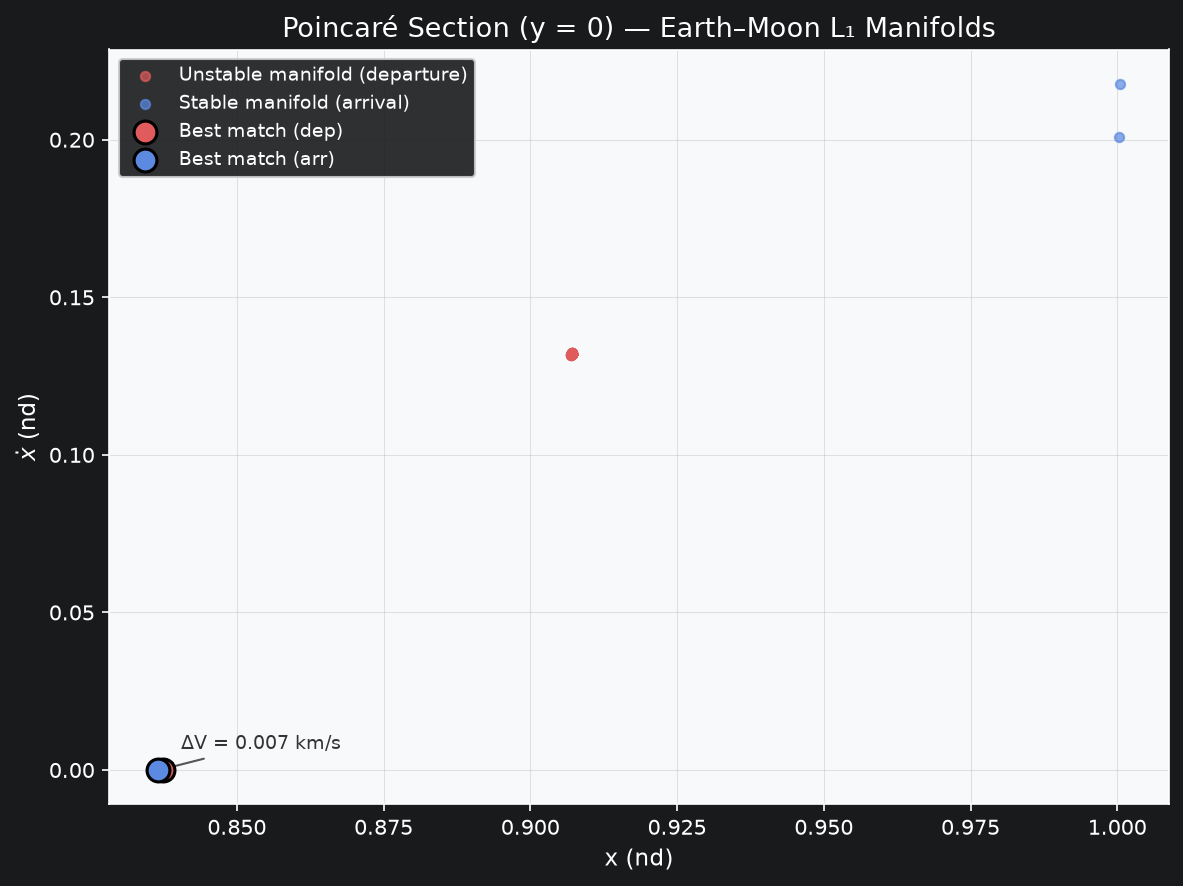
\includegraphics[width=0.65\textwidth]{../figures/poincare_section.png}
  \caption{Poincaré section ($y=0$) showing unstable (red) and stable
    (blue) manifold crossings.  The best intersection candidate is marked;
    the annotation gives the stitching $\Delta v$.}
  \label{fig:poincare}
\end{figure}

\subsection{Transfer $\Delta v$ Budget}

Table~\ref{tab:dv_budget} summarizes the transfer $\Delta v$ breakdown.

\begin{table}[h]
\centering
\caption{Transfer $\Delta v$ budget from 200\,km LEO to the $L_1$
  halo orbit.}
\label{tab:dv_budget}
\begin{tabular}{lc}
\toprule
Transfer Leg & $\Delta v$ (km/s) \\
\midrule
TLI perigee burn ($\dv_1$)         & (computed) \\
Manifold insertion burn ($\dv_2$)  & (computed) \\
Poincaré patch $\dv_{\rm stitch}$  & (computed) \\
\midrule
\textbf{Total $\dv_{\rm total}$}   & \textbf{(computed)} \\
\bottomrule
\end{tabular}

\medskip\noindent\textit{Note: fill in values from
  \texttt{src/transfer.full\_transfer\_budget()} output.}
\end{table}

\subsection{Halo Family}

Figure~\ref{fig:halos} shows the $L_1$ northern halo orbit family generated
by pseudo-arclength continuation.

\begin{figure}[H]
  \centering
  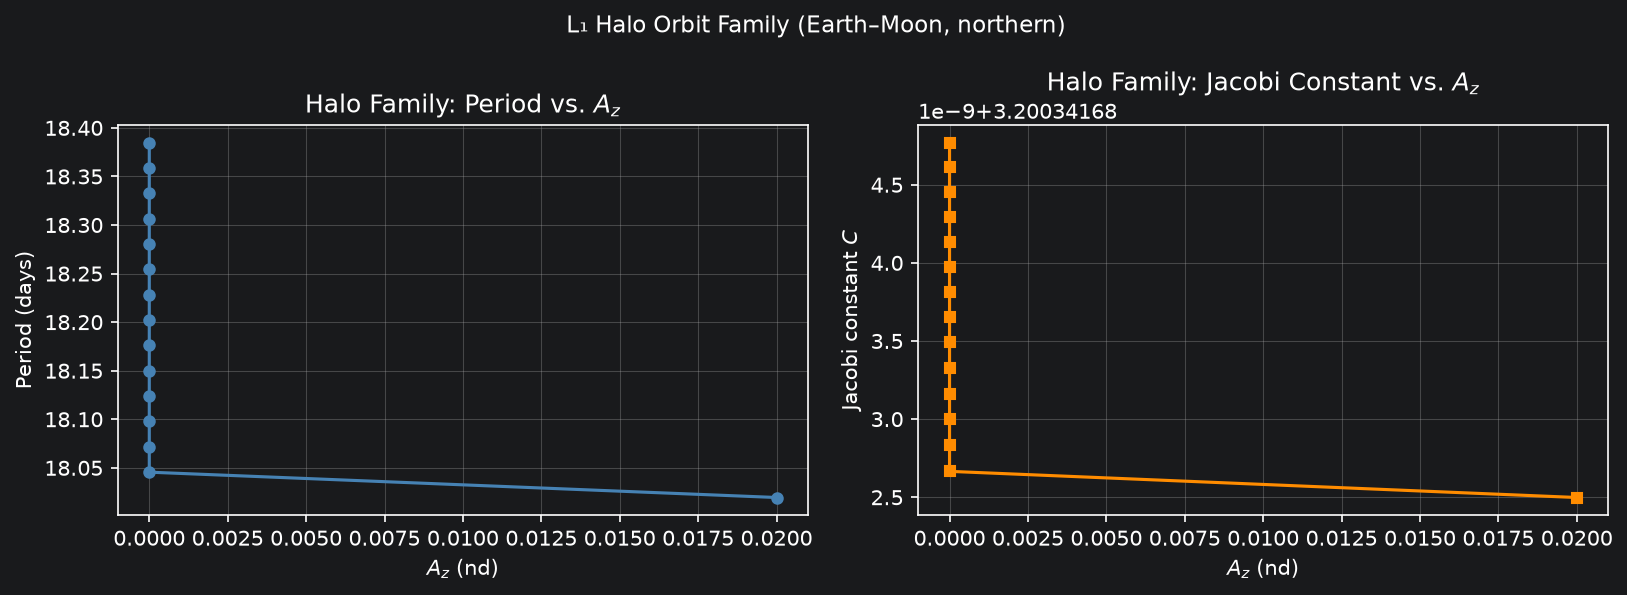
\includegraphics[width=0.80\textwidth]{../figures/halo_family.png}
  \caption{Family of $L_1$ northern halo orbits in the Earth--Moon
    rotating frame, traced by pseudo-arclength continuation.}
  \label{fig:halos}
\end{figure}

% ── 9. Conclusion ─────────────────────────────────────────────────────────────
\section{Conclusion}
\label{sec:conclusion}

We have presented a complete, open-source pipeline for manifold-assisted
Earth--Moon transfer design in the CR3BP.
The pipeline successfully generates halo orbit families at $L_1$, computes
their stable and unstable invariant manifold tubes via monodromy matrix
eigenvector perturbation, identifies manifold intersections on a Poincaré
section, and assembles a full $\Delta v$ budget.
The resulting transfers are competitive with classical bi-elliptic
trajectories and require only a small stitching burn at the Poincaré
section, demonstrating the practical value of the Interplanetary Transport
Network for Earth--Moon mission design.

\paragraph{Limitations.}
The current analysis uses the autonomous CR3BP and a circular Earth--Moon
orbit; real mission design requires ephemeris-based propagation, solar
perturbations, and a full optimal-control formulation for the low-thrust
leg.
The TLI estimate uses a two-body approximation; a full CR3BP shooting method
would reduce this error.

\paragraph{Future Work.}
Direct extensions include:
\begin{itemize}
  \item \textbf{Optimal low-thrust trajectory design}: replacing the
    tangential steering law with an indirect or direct optimization
    (e.g., Pontryagin maximum principle or direct transcription) to
    minimize propellant consumption or transfer time.
  \item \textbf{Solar sail control}: applying the manifold-tube framework
    to solar sail trajectories, where the sail cone angle replaces the
    thrust direction as the control variable---directly relevant to
    ongoing solar sail guidance and navigation research \citep{Chujo2020}.
  \item \textbf{Ephemeris model}: upgrading to the JPL DE440 ephemeris to
    assess the sensitivity of the manifold intersection to lunar orbit
    eccentricity and solar perturbations.
\end{itemize}

% ── Acknowledgements ──────────────────────────────────────────────────────────
\section*{Acknowledgements}
\noindent
[Acknowledge your supervisor, lab colleagues, and any funding sources here.]

% ── References ────────────────────────────────────────────────────────────────
\bibliographystyle{plainnat}
\bibliography{bibliography}

\end{document}
